% !TEX TS-program = pdflatex

\documentclass[unicode,11pt,notheorems,xcolor=table]{beamer}
\usepackage{fix-cm}
\usepackage[T2A]{fontenc}
\usepackage[utf8]{inputenc}
\usepackage[russian]{babel}
\usepackage{amsmath,amsfonts,amssymb,amsthm}
\usepackage{mathtools}
\usepackage{diagbox}

\usepackage{ulem}
\usepackage{tikz}
\usepackage{graphicx}
\usepackage{pgfplots}
\pgfplotsset{compat=1.16}

\usetikzlibrary{matrix,arrows,decorations.pathmorphing, arrows.meta,positioning}
\usetikzlibrary{positioning,calc}
\usetikzlibrary{patterns}
\usetikzlibrary{decorations.pathreplacing}

%Описание стиля презентации
\usetheme[sidebar=0]{kfmn} 
\setbeamercovered{transparent}

%\definecolor{cyan}{RGB}{240,217,1}
%\definecolor{vgugreen}{RGB}{143,188,103}
%\definecolor{vgured}{RGB}{234,38,40}
%\definecolor{vgublue}{RGB}{53,101,167}
\hypersetup{colorlinks,linkcolor=,urlcolor=blue}

\makeatletter
	\g@addto@macro{\endtabular}{\rowfont{}}% Clear row font
	\makeatother
	\newcommand{\rowfonttype}{}% Current row font
	\newcommand{\rowfont}[1]{% Set current row font
		\gdef\rowfonttype{#1}#1\ignorespaces%
	}
\makeatother

\newcommand{\myunit}{9mm}
\tikzset{
    node style sp/.style={draw,circle,minimum size=\myunit},
    node style ge/.style={circle,minimum size=\myunit},
    arrow style mul/.style={draw,sloped,midway,fill=white},
    arrow style plus/.style={midway,sloped,fill=white},
}

%[0, 6, 8, 8, 10, 5, 6, 10, 8, 10, 10], 

\pgfdeclareimage[height=8mm]{university-logo}{logo-iem.png}
\logo{\pgfuseimage{university-logo}}
%2[0, 11, 10, 8, 11, 5, 11, 11, 8, 11, 10, 11],

\titlepicture{
	\begin{tikzpicture}[y=1.4cm,overlay,rotate=8]
	\coordinate (O) at (-3cm,0.9cm);
	\filldraw[thick,draw= vgublue, fill=vgublue!20!white] (0,0) circle[radius=4.2cm];
	\clip (0,0) circle[radius=4.2cm];
	\draw (-1.5,1.5) node{
	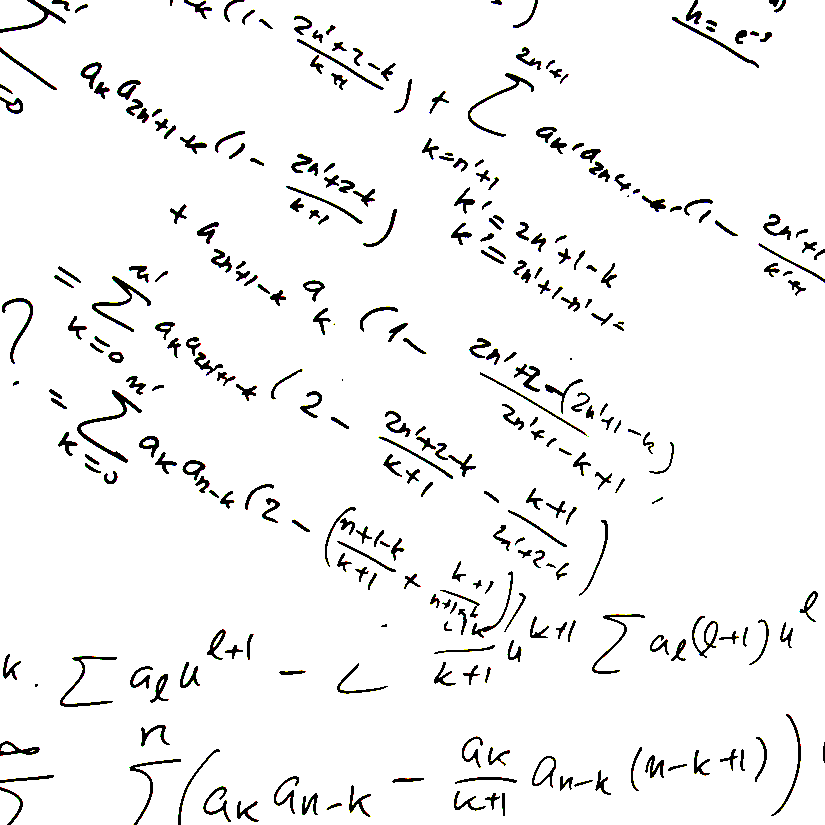
\includegraphics[width=8cm]{titlepic.png}
	};
\end{tikzpicture}
}

\usepackage[math]{iwona}

\newcommand{\hplus}{\mathbin{\hat+}}
\newcommand{\hdot}{\mathbin{\hat\cdot}}
% Описание теорем
\newtheorem{theorem}{Теорема}
\newtheorem{seq}{Следствие}
%%

\LECT % 

% Титульный лист теорем
\author[Д.\,В. Чупраков]{канд.\,физ.-матем.\,наук, доцент Д.\,В. Чупраков\\[6pt] usr10381@vyatsu.ru}

\institute[ВятГУ]{ФГБОУ ВО Вятский государственный университет}

\department{Факультет экономики и финансов}

\title[Лекция~22. Матричные игры -- 1]{
	Введение в экономико-математическое моделирование\\[12pt]
	Лекция~22. Матричные игры}
\date{9 декабря 2020~г.}


\setbeamercovered{invisible}

\setbeamercolor{math text}{fg=vgured!70!black}

\pgfmathdeclarefunction{gauss}{2}{%
  \pgfmathparse{1/(#2*sqrt(2*pi))*exp(-((x-#1)^2)/(2*#2^2))}%
}
\begin{document}


\maketitle

 \begin{frame}{Структура лекции}{}
 	\tableofcontents
 \end{frame}

\section{}

\begin{frame}{}{}
    \begin{itemize}
        \item Первая значительная книга по теории игр появилась в 1944г (Дж. фон Нейман, С. Моргенштерн «Теория игр и экономическое поведение»). 
        \item В 1994 г. за успехи в развитии теории игр трем ученым J.F. Nash, J.C. Harsanyi и R. Selten была присуждена премия имени Альфреда Нобиля.
        \item Теория игр она нашла свое применение, прежде всего, в военном деле, политике, юриспруденции, психологии, биологии и экономике.
    \end{itemize}
\end{frame}

\begin{frame}{}{}
    Моделями теории игр можно описать экономические, правовые, классовые, военные конфликты, взаимодействие человека с природой.

    Все такие модели в теории игр принято называть играми.
\end{frame}



\begin{frame}{Постановка задачи матричной игры}{}
    \begin{itemize}
        \item пусть имеются две стороны $A$ и $B$;
        \item сторона $A$ имеет~$m$ стратегий игры, а сторона $B$~--- $n$ стратегий;
        \item Выигрыш стороны $A$ при выборе ею стратегии $A_i$, а стороной $B$~--- стратегии $B_j$, составляет $a_{ij}$;
        \item Проигрыш стороны $B$ в этом случае составляет также $a_{ij}$;
        \item Сторонам известны стратегии обеих сторон и все возможные выигрыши;
        \item Сторонам неизвестно какой стратегии будет придерживаться другая сторона, 
        \item Известен принцип, по которому обе стороны выбирают оптимальные для себя стратегии.
    \end{itemize}

\end{frame}


\begin{frame}{}{}

\end{frame}


\begin{frame}{Принцип доминирования}{}
    \begin{description}
        \item[Цель.] Уменьшить размерность задачи (редуцировать платежную матрицу).
        \item[Идея.] исключить из рассмотрения те стратегии игроков, которые являются очевидно не выгодными для игроков.
    \end{description}
    Такой столбец (стратегию) называют строго доминирующим остальные столбцы.

\end{frame}


\begin{frame}{}{}

\end{frame}


\begin{frame}{}{}

\end{frame}


\begin{frame}{}{}

\end{frame}


\begin{frame}{}{}

\end{frame}


\begin{frame}{}{}

\end{frame}


\begin{frame}{}{}

\end{frame}


\begin{frame}{}{}

\end{frame}


\begin{frame}{}{}

\end{frame}


\begin{frame}{}{}

\end{frame}


\begin{frame}{}{}

\end{frame}


\begin{frame}{}{}

\end{frame}



\end{document}